\section{Architectural Design}
\subsection{Overview: high-level components and interactions}
\begin{figure}[H]
    \begin{center}
        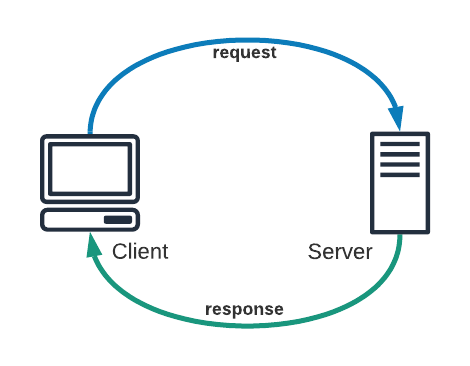
\includegraphics[width=\textwidth/2]{img/Client-Server.png}
        \caption{Client-Server paradigm}\label{client_server_par}
    \end{center}
\end{figure}

As figure \ref{client_server_par} represents, the system is a distributed application which follows the common known client-server paradigm.

In particular, there are two different types of client-server interactions, because the product has 2 modules that need to fulfill different goals for different actors. 

Since Module 1 will feature a mobile application, that will contain an internal database in order to make it less dependent from the server. This aspect makes it a more of a thick client.

Module 2, on the other hand, will feature a \textit{Web Application}, which is by definition a thin client, because of its total dependency from the server.
This type of client does not contain the application business logic, but only the presentation layer.

In both cases the server is \textit{fat} and contains all the data management and business logic.

In this section the architecture will be described in an easy way, justifying all the choices for adopted patterns.

\begin{figure}[H]
    \begin{center}
        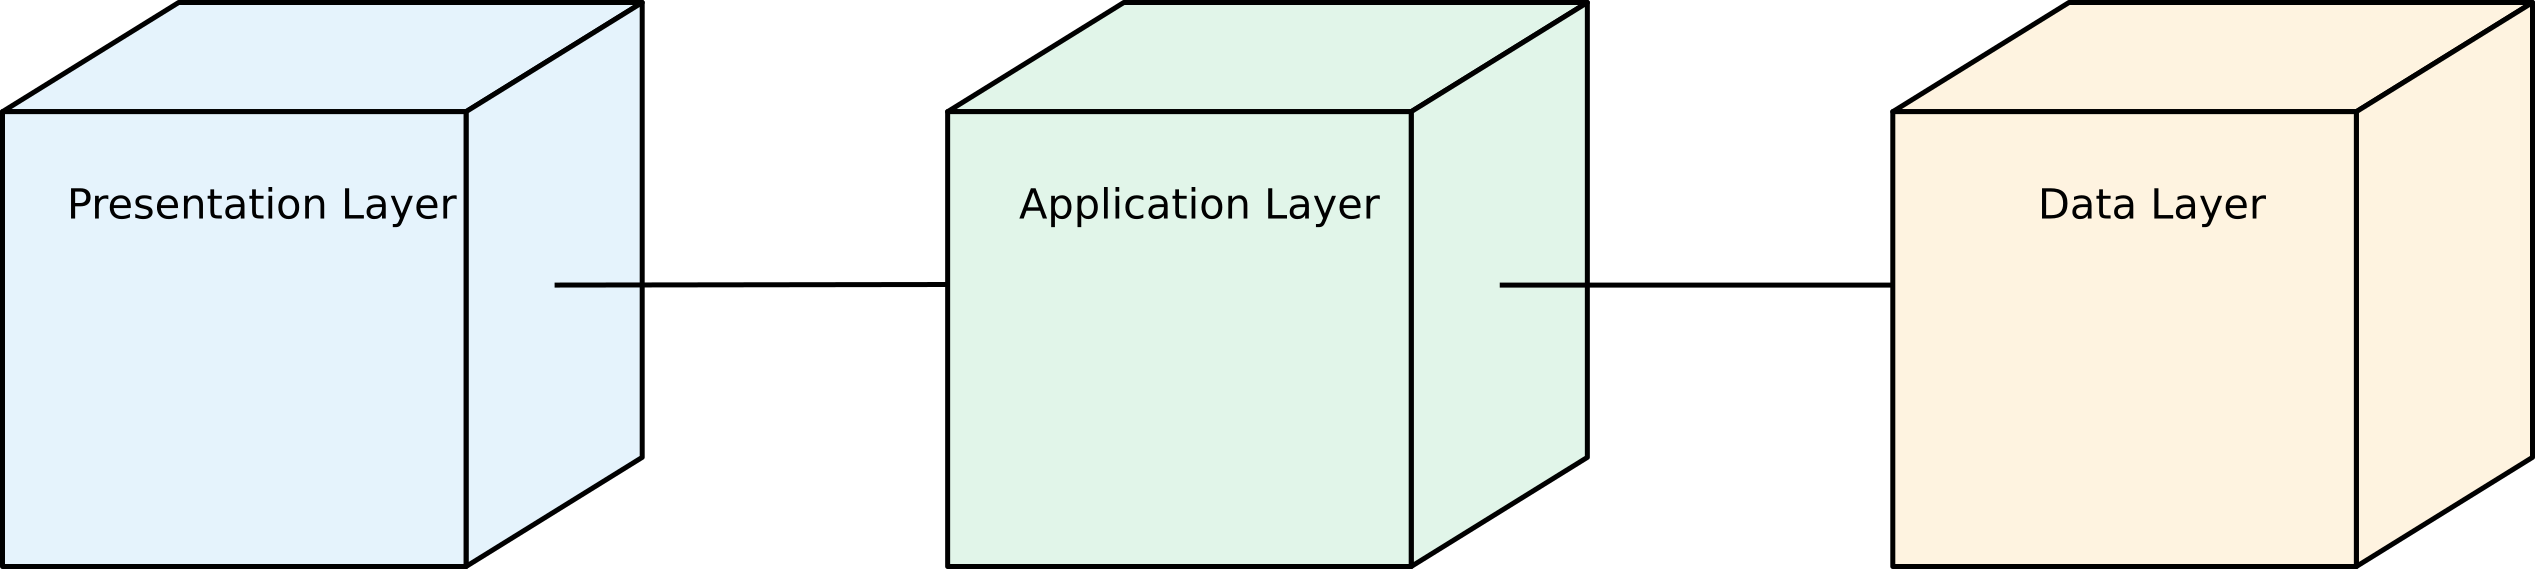
\includegraphics[width=\textwidth]{img/3-tier.png}
        \caption{Three layers application}\label{three_tier_desc}
    \end{center}
\end{figure}

In figure \ref{three_tier_desc} the three S2B layers are shown, which respectively are:
\begin{itemize}
    \item \textbf{Presentation Layer:} it manages the presentation logic and, consequently, all the interactions with the end user. This is also called \textit{rendering layer}.
    \item \textbf{Application (Logic) Layer:} it manages the business functions that the S2B must provide.
    \item \textbf{Data Layer:} it manages the safe storage and the relative access to data.
\end{itemize}

As shown in the high level representation of figure \ref{architecture_overview} the S2B is divided into three layers that are physically separated by installing them on different tiers. A tier is a physical (or a set of) machine, each of them with its own computational power.

The application described in this document is composed by four tiers.

\begin{figure}[H]
    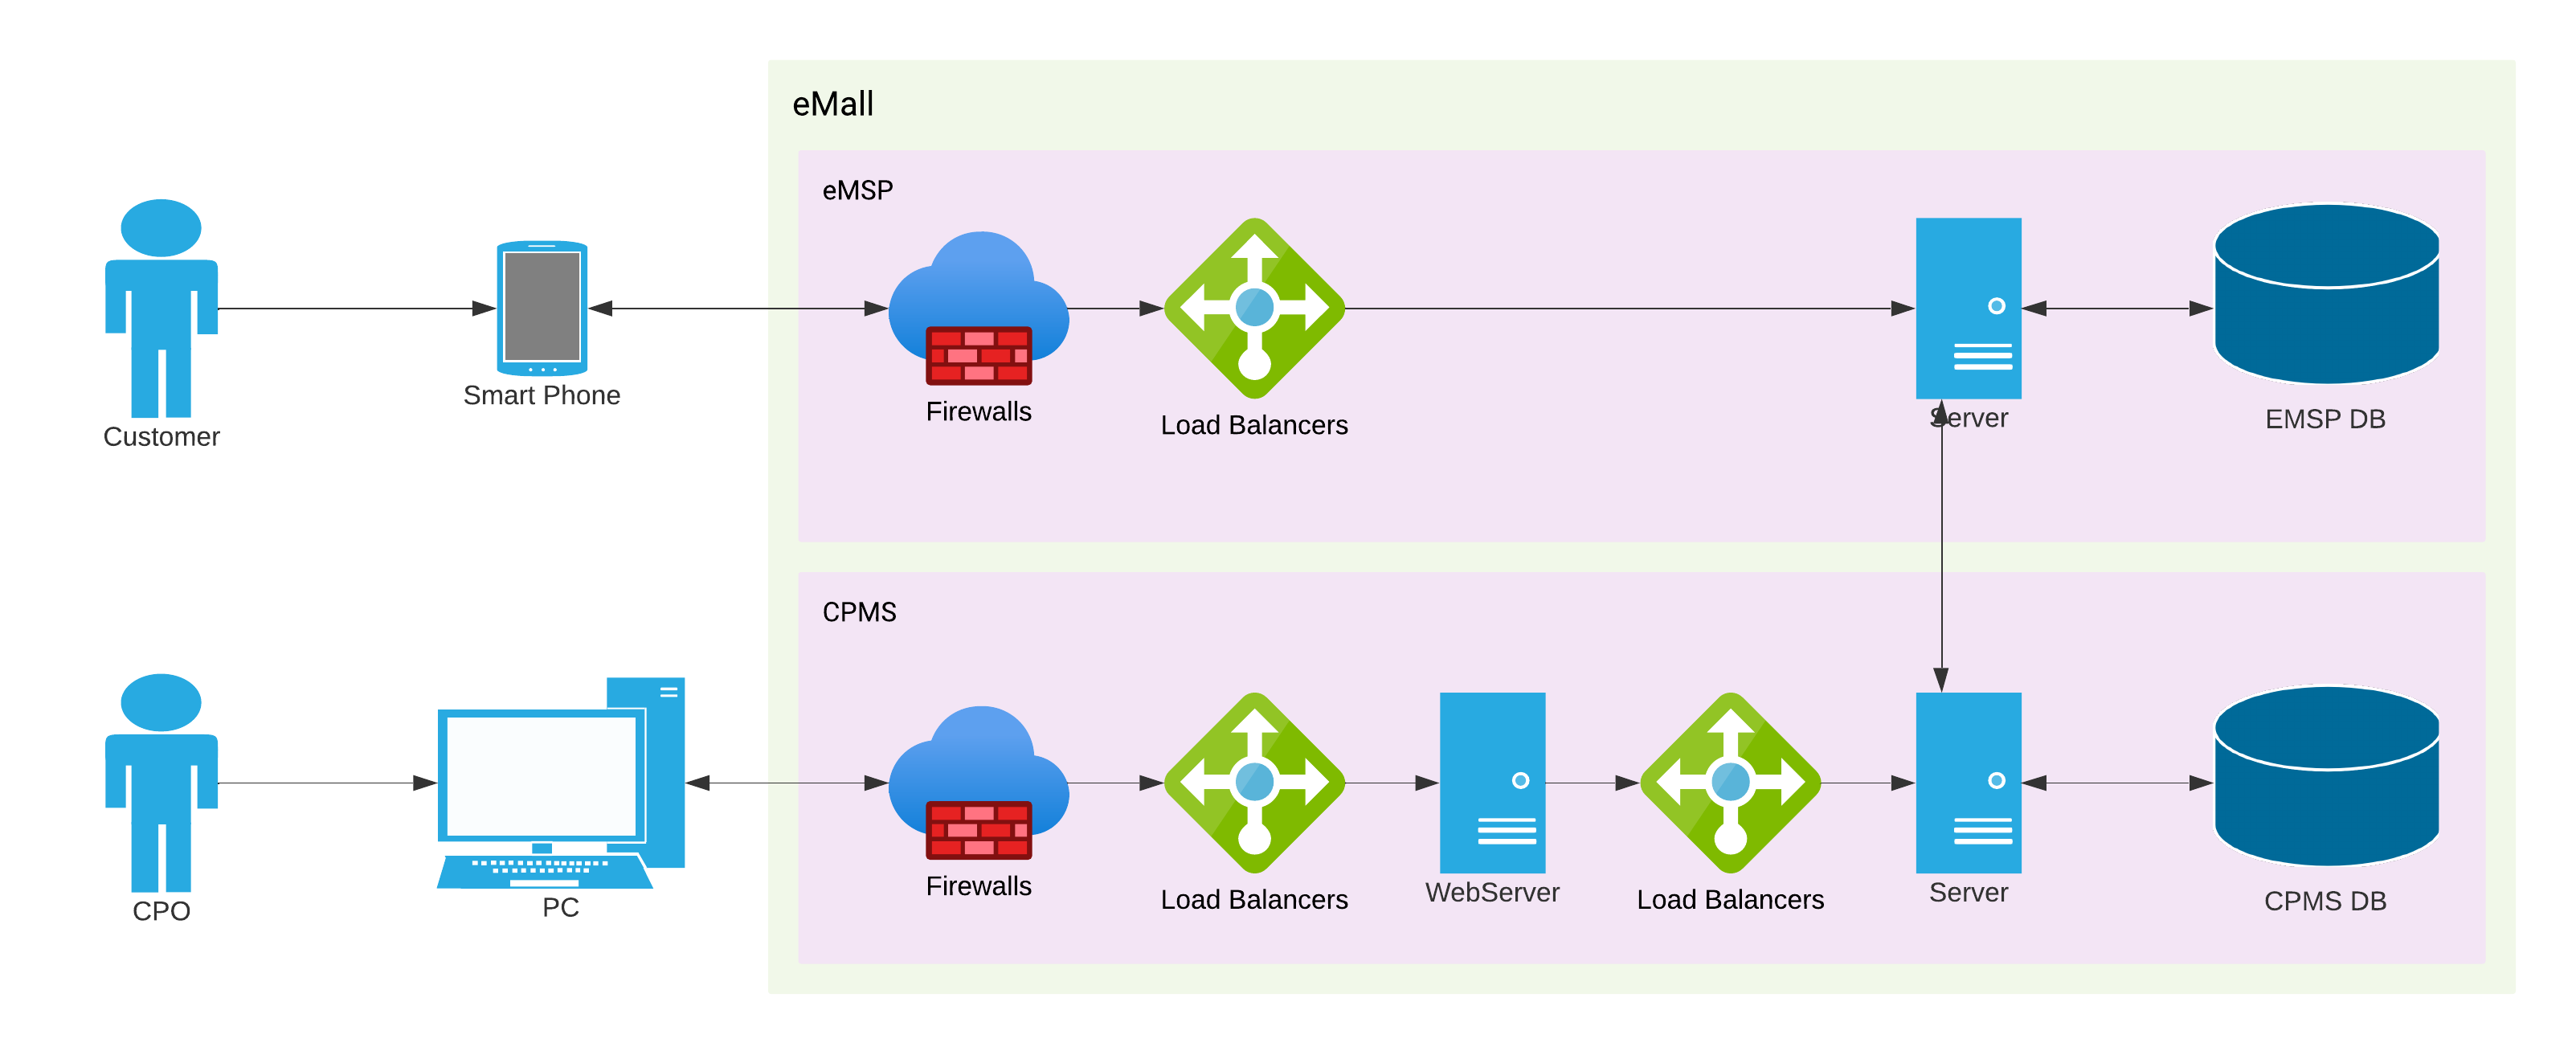
\includegraphics[width=\textwidth]{img/ArchitectureOverview.png}
    \caption{Architecture of the application}\label{architecture_overview}
\end{figure}    


\subsection{Component view}

In this section there is an high-level analysis of the main components and their subcomponents. Main interfaces interactions between components are also provided.

\begin{figure}[H]
    \begin{center}
        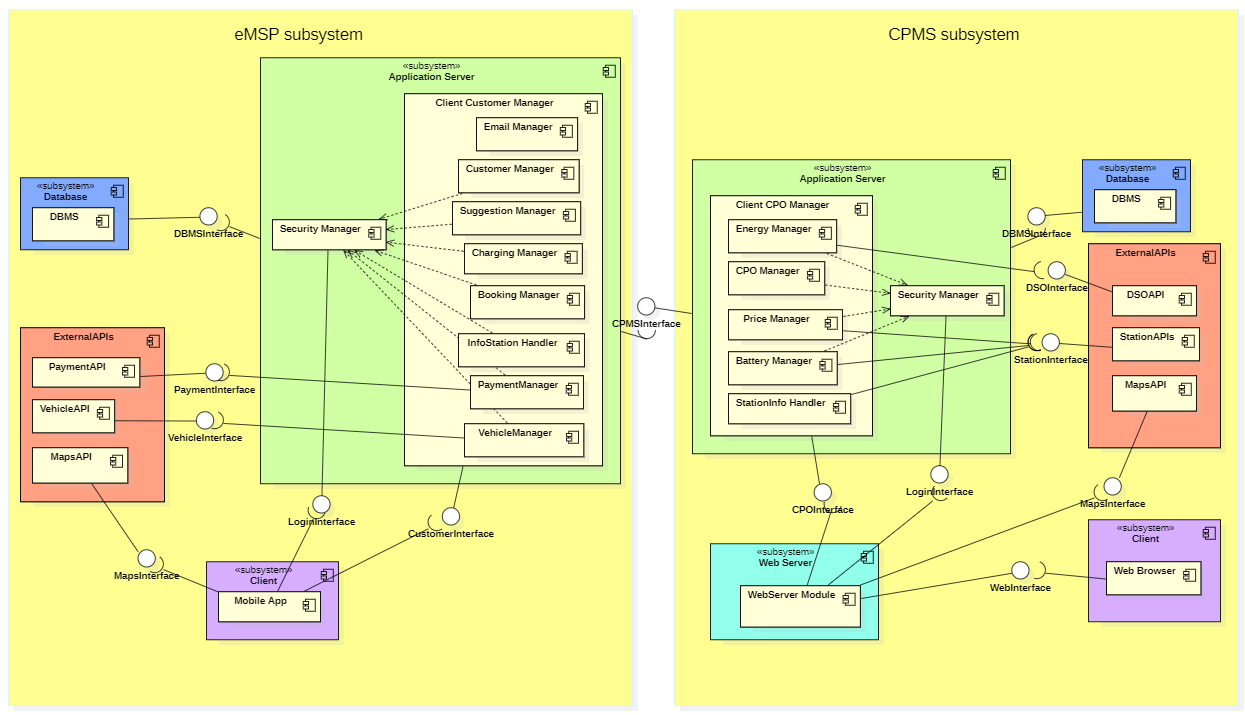
\includegraphics[width=\textwidth]{img/ComponentDiagram.PNG}
        \caption{Component Diagram}\label{component_diagram}
    \end{center}
\end{figure}

\begin{itemize}
    \item \textbf{Client Customer Manager}\\This module handles all the requests made by the client. At the beginning, when the client is not logged in, the module offers (through the customer manager) a LoginInterface which permits to execute a sign up or sign in operation. Once the client has logged in, the module shows only the CustomerInterface which the customer will exploit.
    \item \textbf{Email Manager}\\This component handles the email notifications, such as the sign up and forgot password ones.
    \item \textbf{Customer Manager}\\This module contains all the features in order to manage the customer side. In fact, it includes the log in and sign up manager.
    
    \item \textbf{Suggestion Manager}\\This module manages the push notifications. Based on the information aquired thanks to the Vehicle Manager, it creates suggested bookings and shows all the details about them. It allows also to confirm a suggested booking on the application.
    \item \textbf{Charging Manager}\\ This module manages the charging process operations, such as the socket unlocking. It also shows the remaining time to end a charge and the charging state (in charge/ finished).
    \item \textbf{Booking Manager}\\This component manages the booking process. It aims to handle the sockets' booking and shows the details of the different bookings.
    \item \textbf{InfoStation Handler}\\This component handles the information about the charging stations. So it shows information about sockets types and related prices and special offers, sockets availabity and specifications about the charging stations.
    \item \textbf{Payment Manager}\\This component's aim is to handle the customer payment. It uses a PaymentAPI in order to process the task.
    \item \textbf{Vehicle Manager}\\This component's aim is to get the customer's vehicle information, such as the position, the battery percentage and the calendar.
    \item \textbf{Client CPO Manager}\\This module handles all the requests made by the client. At the beginning, when the client is not logged in, the module offers (through the CPO manager) a LoginInterface which permits to execute a sign in operation. Once the client has logged in, the module shows only the CPOInterface which the CPO will exploit.
    \item \textbf{Energy Manager}\\This module's aim is to handle the energy options.
    It also allows to select a DSO and aquire energy from it. On the other hand allows to set some operations such as the auto-mode.
    \item \textbf{CPO Manager}\\This module contains all the features in order to manage the user side. It includes the log in manager.
    \item \textbf{Price Manager}\\This module in needed to set special offers on socket's types in selected charging stations. Moreover it is used to set socket prices.
   
    \item \textbf{Battery Manager}\\This component manages the battery in the charging stations. It handles the battery policy change.
    \item \textbf{StationInfo Handler}\\This component handles the information about the charging stations. So it shows information about sockets types and related prices and special offers, sockets availabity and specifications about the charging stations.
 
    \item \textbf{Security Manager}\\Finally, this components handles all the security issues of the S2B. In fact, its aim is to authenticate and authorize requests, relying on the token provided from the client (since it should be a REST application). If a request is not authenticated, it takes the user to a login page; otherwise it simply replies with an unauthorized state message.
\end{itemize}

\subsection{Deployment view}

\begin{figure}[H]
    \begin{center}
        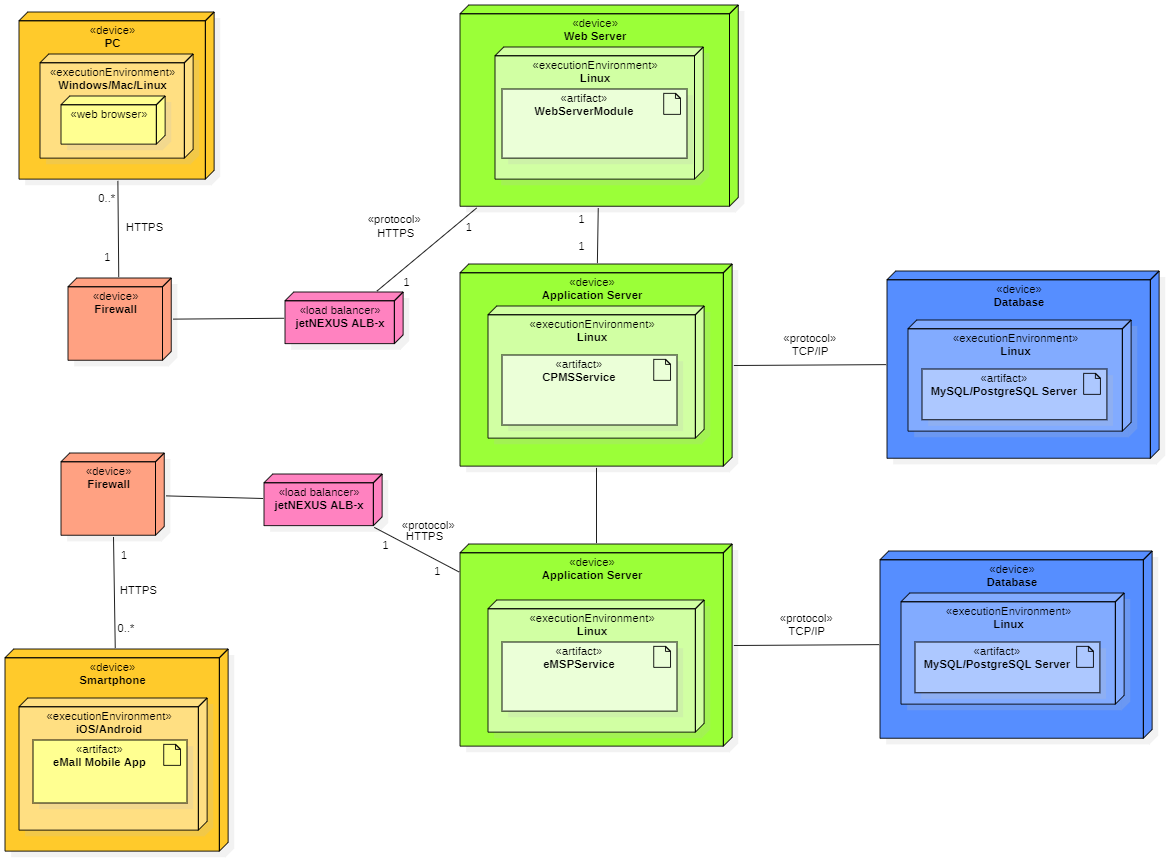
\includegraphics[width=\textwidth]{img/DeploymentDiagram.PNG}
        \caption{Deployment Diagram}\label{deployment_diagram}
    \end{center}
\end{figure}

The deployment diagram in figure\ref{deployment_diagram} shows the needed components for a correct system behavior and the protocols to communicate. As shown in the above image, firewalls and load balancers manage the data stream
from the devices to the servers. First of all, firewalls are in charge of filtering packets
received from the Internet. Then, the packets pass through the load balancer, where
the workload is distributed among the available resources to increase capacity and
reliability.
Each device has its own Operating System where the software runs.
The tiers in the image are the following:
\begin{itemize}
    \item \textbf{Tier 1:} it is the client machine, which can be a computer with a web browser (running, for example, on Windows 10 OS) or the downloadable mobile application (available on both Apple's store and Google's Store).
    \item \textbf{Tier 2:} it includes the replicated web servers, which do not execute any business logic, but simply receive requests from the client, route them to the application servers and serve an HTML file fo the client, which will build the page thanks to client-side scripting. They also append the styling logic of the page (CSS sheets, JS sheets, etc.).
    \item \textbf{Tier 3:} it contains the application servers, which run the core functionalities of the S2B. The whole application layer is mapped into this tier, which communicates to the client tier through APIs, which will be used from the web servers (in case of webapp) and the native application (in case of mobile app download). Furthermore, it communicates to the data tier through the DBMS gateway.
    \item \textbf{Tier 4:} it is composed by the DBMS servers. They store the data and execute actions on it, according to the instruction given by the application servers.
\end{itemize}
\subsection{Runtime view}
As stated previously, Module 1 (eMSP subsystem) is a mobile app while Module 2 (CPMS subsystem) is a web app. All the following diagrams represent the runtime view from the mobile app’s perspective, in order to increase readability, the web app’s perspective isn’t shown as it only differs from the other one by using the web server’s module before calling the Application Server.\\
Every interface uses the REST API through HTTP GET or/and POST calls.
\subsubsection{Signup Customer}
\begin{figure}[H]
    \begin{center}
        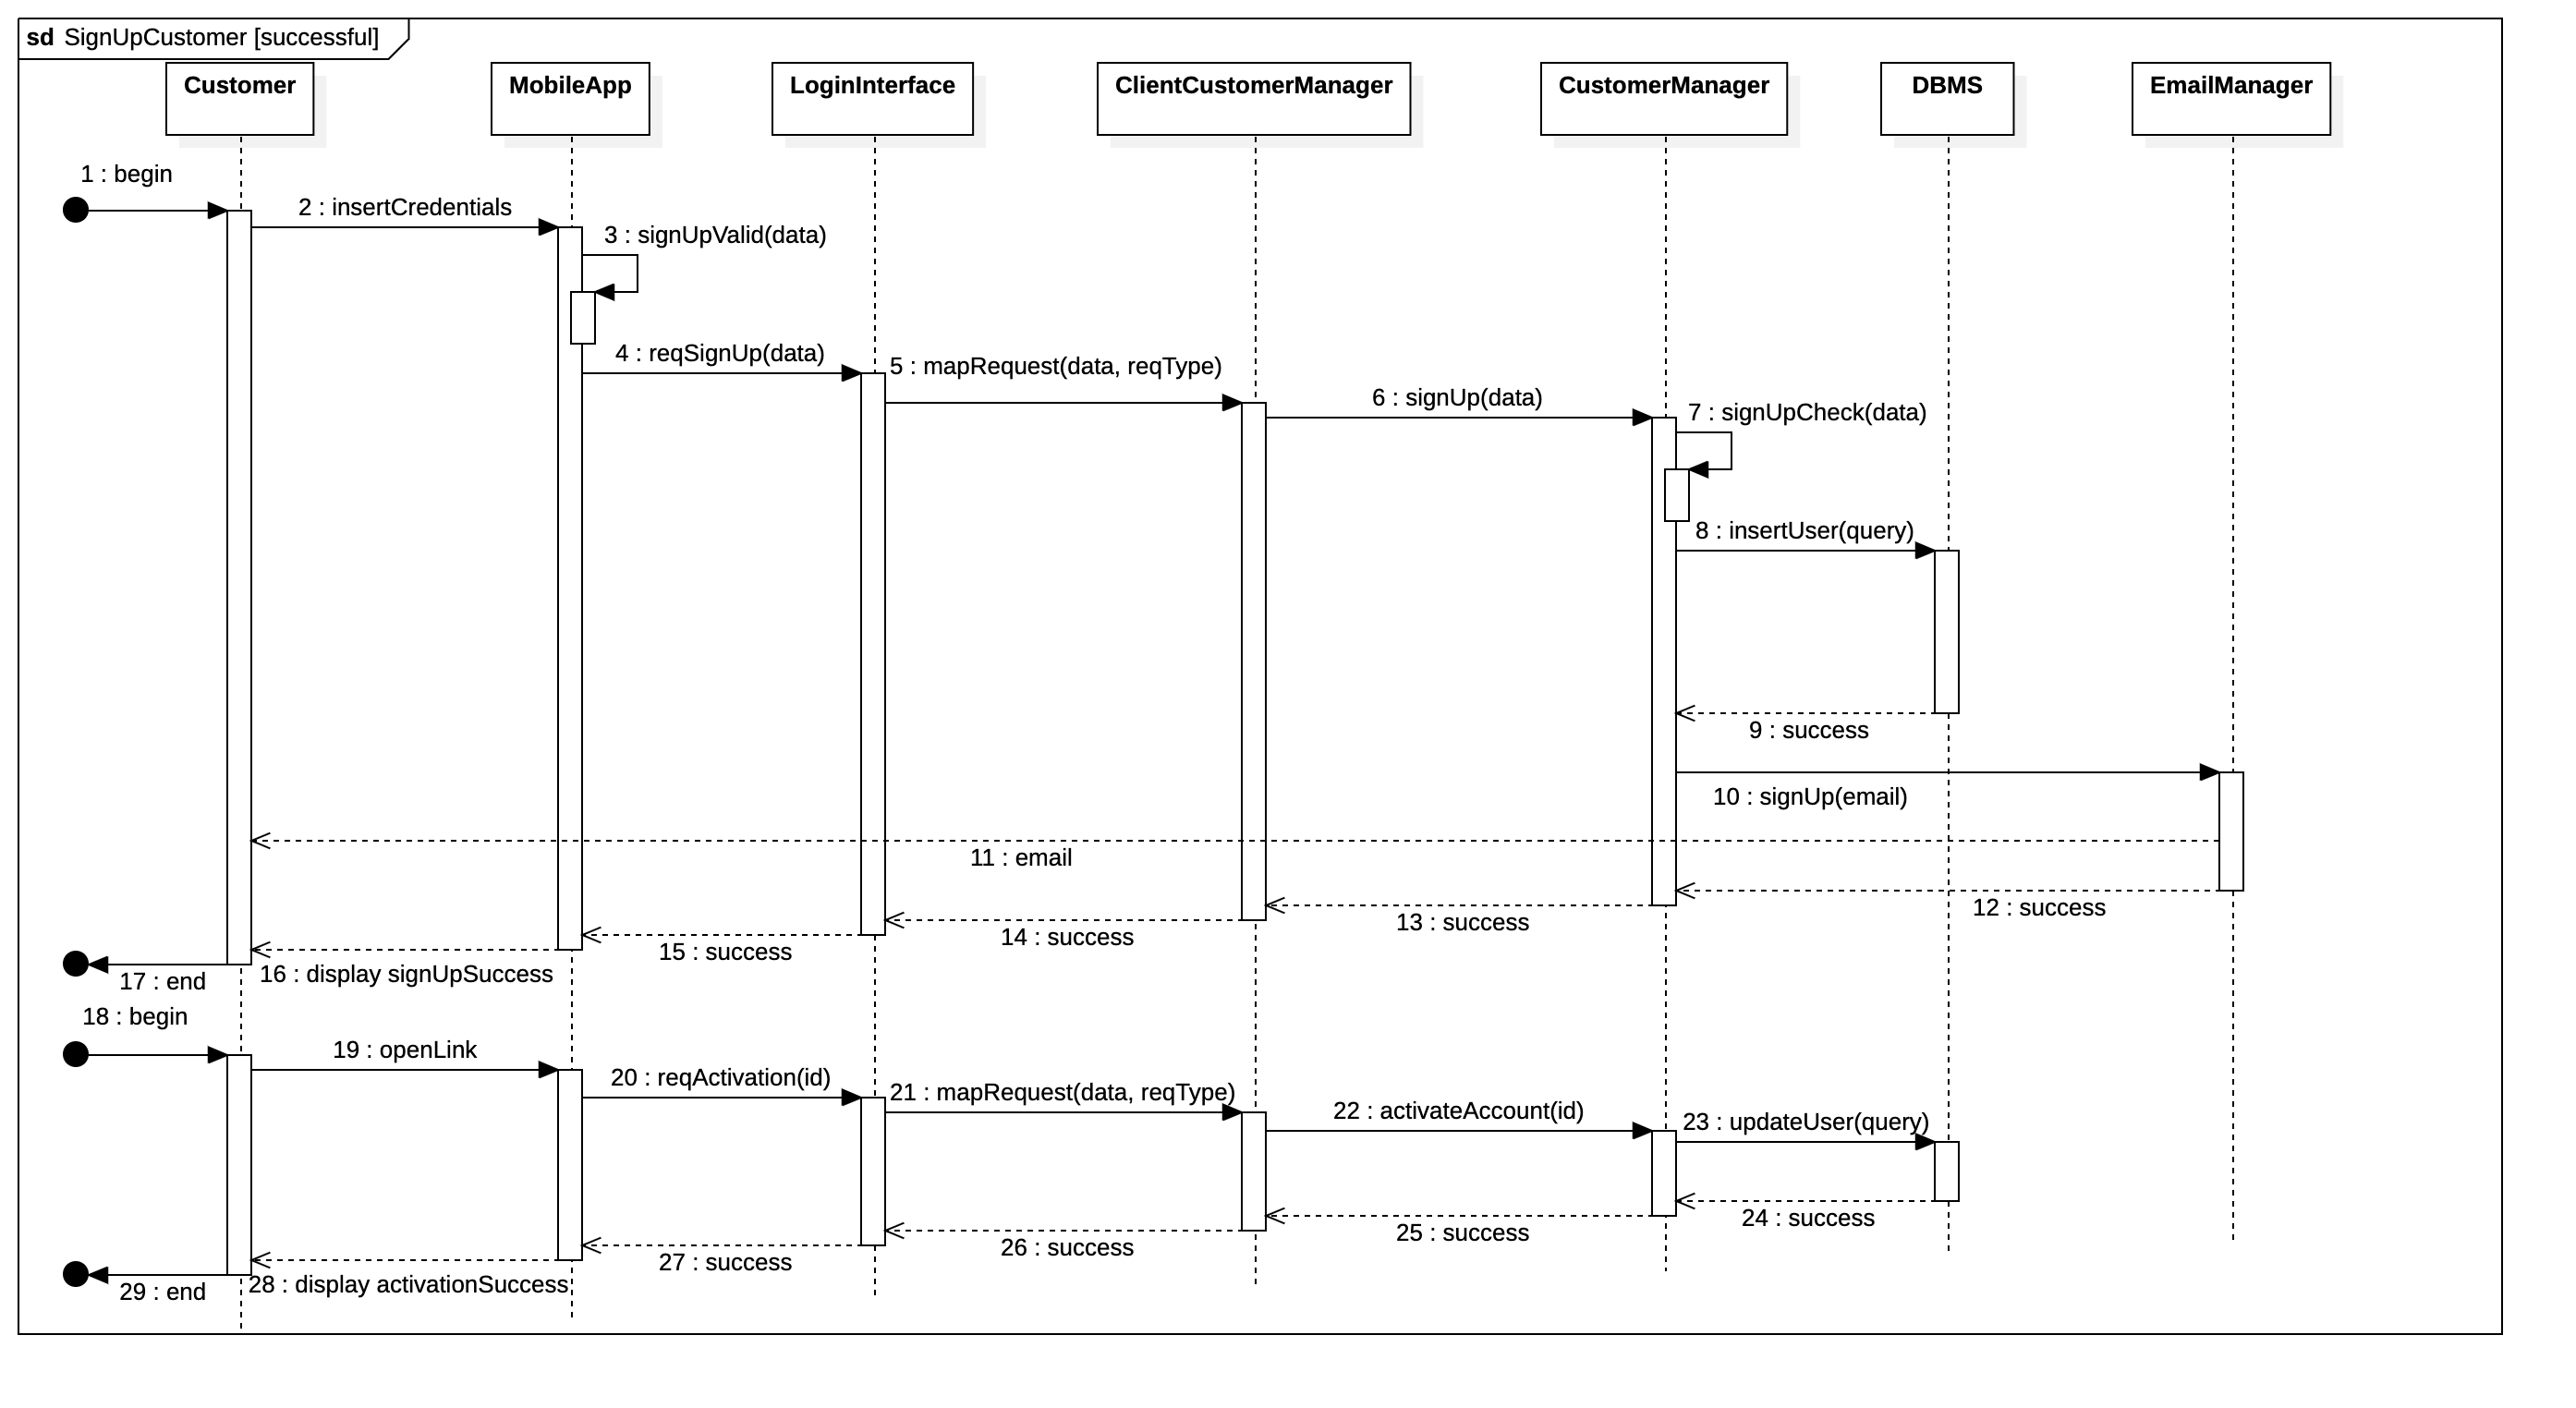
\includegraphics[width=\textwidth]{img/runtime/cust_signup_success}
        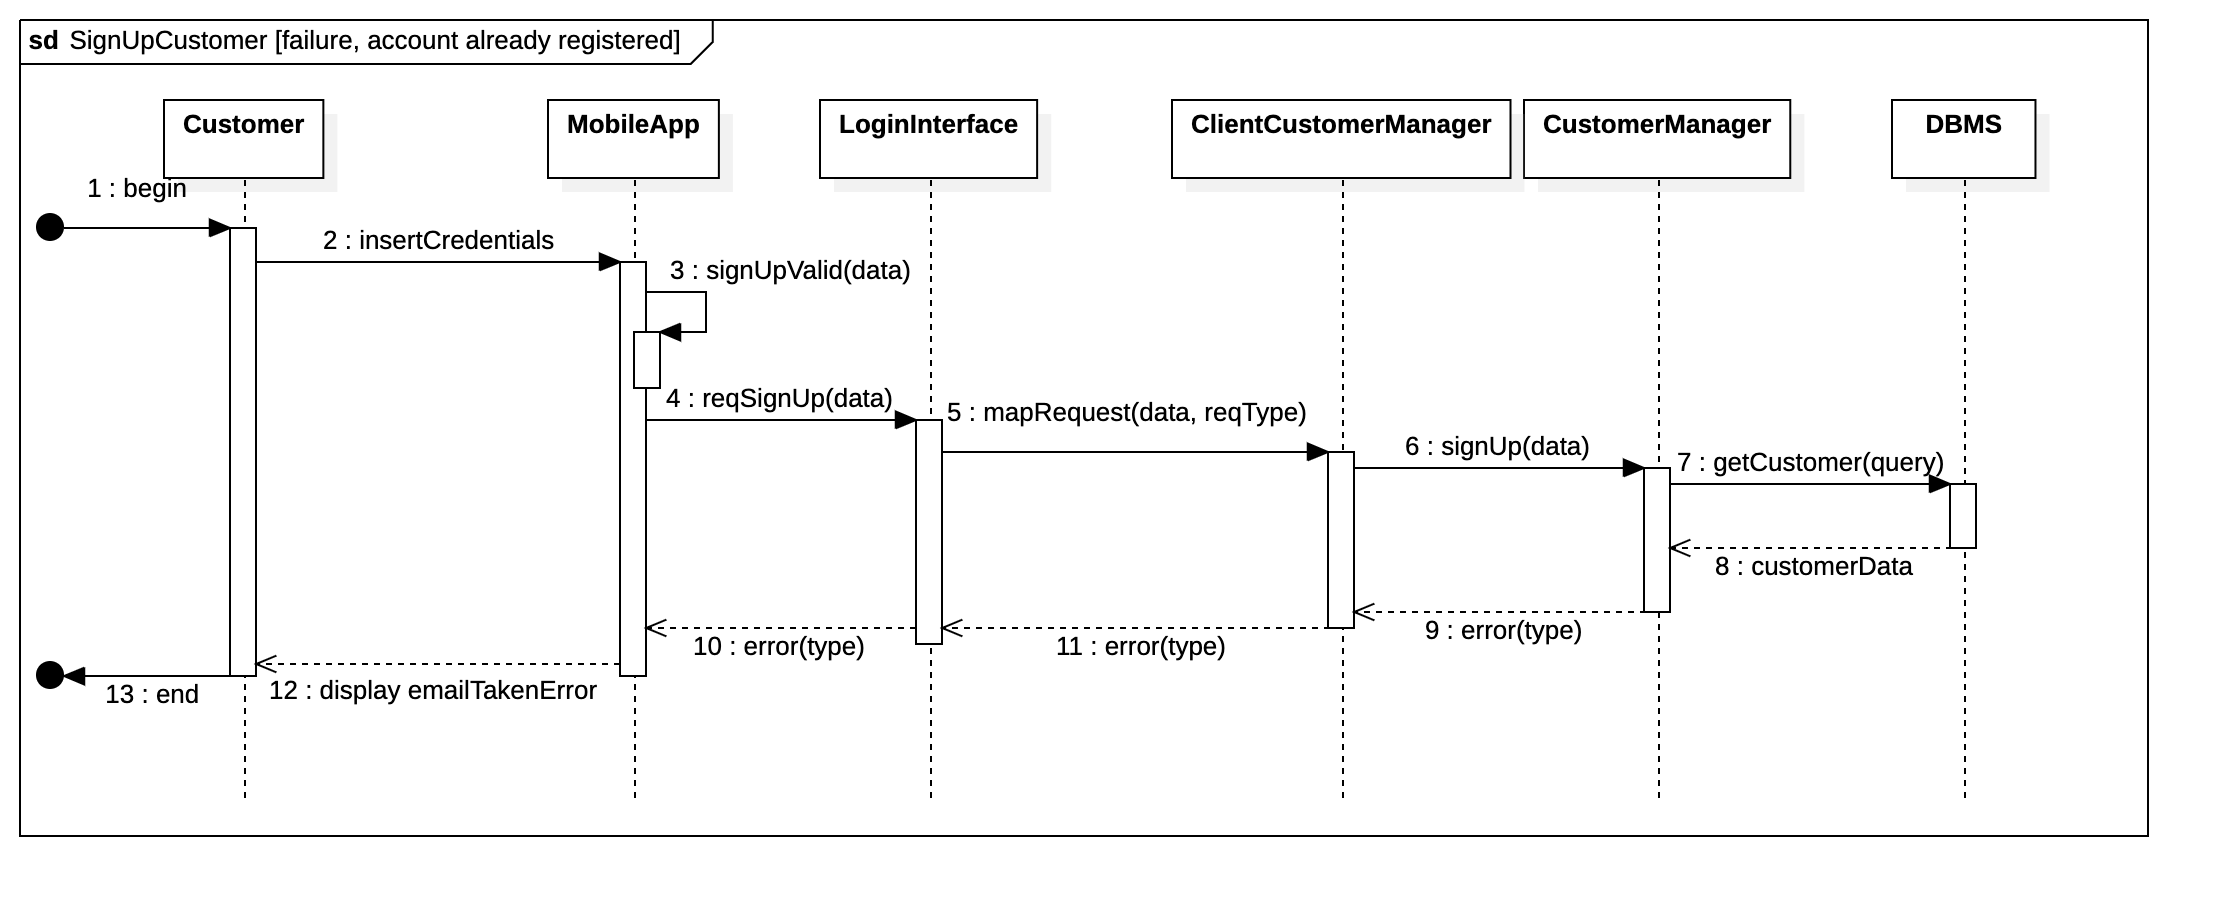
\includegraphics[width=\textwidth]{img/runtime/cust_signup_error}
    \end{center}
\end{figure}
The diagram above represents the process of signing up a Customer. There two possible situations:
\begin{itemize}
\itemize Customer performs a correct registration process;
\itemize Customer performs a wrong registration process (such as the account is already registered or the email in not valid).
\end{itemize}
The Customer begins by inserting his registration credentials in the app. Afterwards the app sends the request to the ClientCustomerManager through the LoginInterface, accessing later the CustomerManager.\\
The CustomerManager checks for the correctness of the received information and if correct it passes it ultimately to the DBMS. Then an email is sent to the Customer by the EmailManager. If the CustomerManager checks fail, the user is sent a specific error message related to his issue.
\subsubsection{Login Customer}
The Customer inputs his login credentials and then the MobileApp sends the request, through the LoginInterface to the ClientCustomerManager, which forwards them to the CustomerManager that checks for their correctness and then interrogates the DBMS and searches for the credentials. If the returned value is null the ClientManager sends a specific error message and the login fails, otherwise a 200 response status code is sent to the MobileApp.
\subsubsection{Signup Customer}
\subsubsection{Signup Customer}

\subsection{Component interface}


\begin{figure}[H]
    \begin{center}
        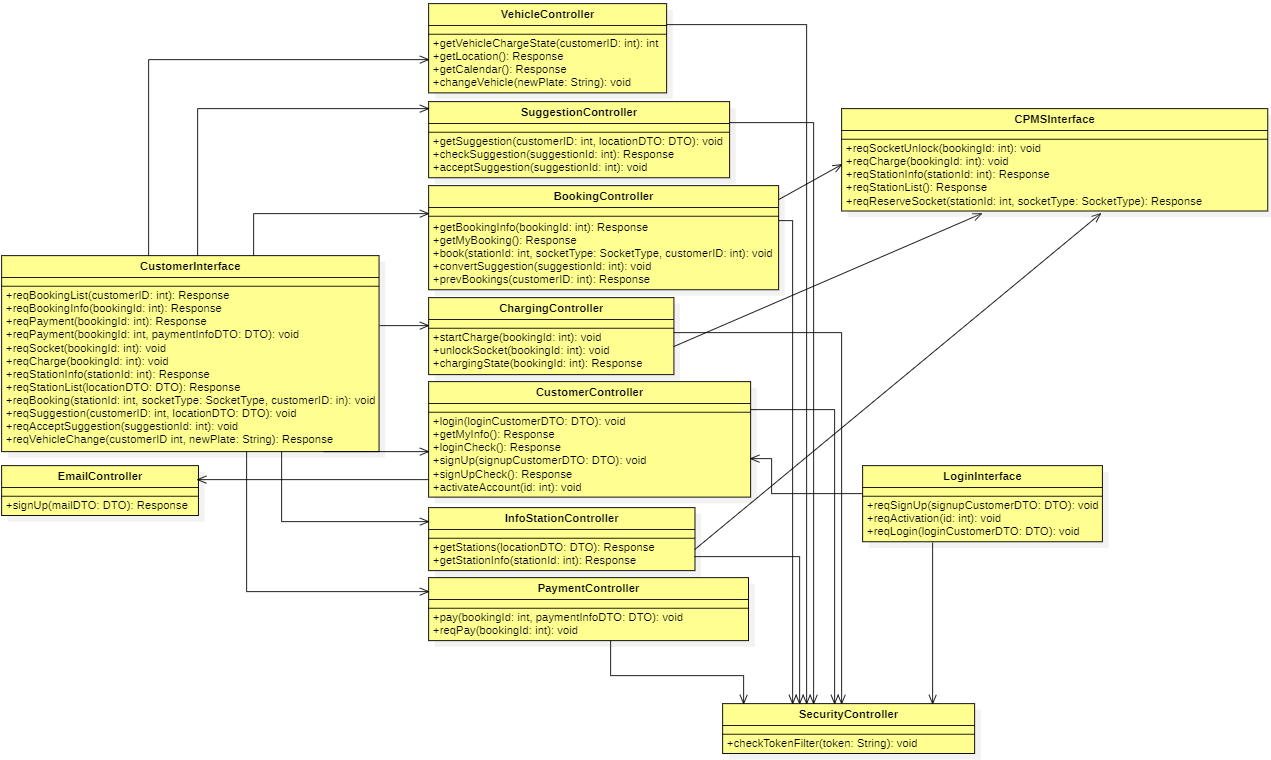
\includegraphics[width=\textwidth]{img/ComponentInterface1.PNG}
        \caption{Component Interface 1}\label{component_interface1}
    \end{center}
\end{figure}

\begin{figure}[H]
    \begin{center}
        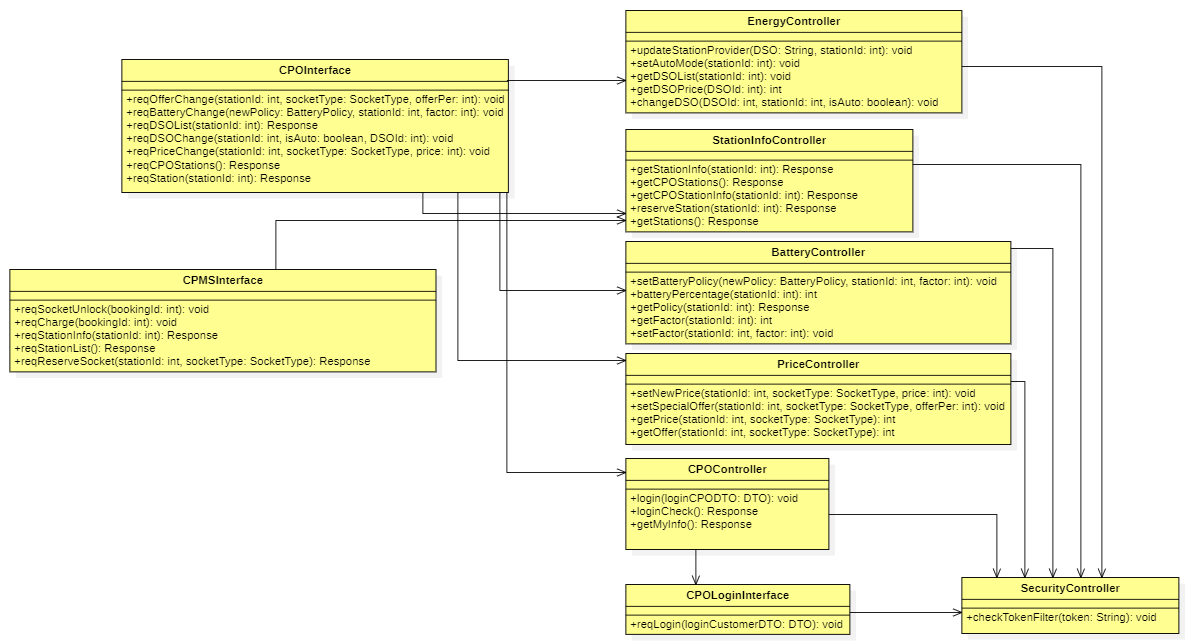
\includegraphics[width=\textwidth]{img/ComponentInterface2.PNG}
        \caption{Component Interface 2}\label{component_interface2}
    \end{center}
\end{figure}

\subsection{Selected architectural styles and patterns}

\subsubsection{Four-tiered architecture}
We chose this architecture for many reasons:
\begin{itemize}
    \item \textbf{Flexibility:} Once the interfaces of the S2B are defined, then the interior logic is independent from outside. Single components can therefore be implemented in parallel. And can be modified without affecting the system.
    \item \textbf{Scalability:} An application divided on several tiers guarantees that the approach of scaling the architecture is adopted only for the most critical components. The result obtained maximizes the performance but also minimizes the costs.
    \item \textbf{Load Distribution:} the presence of several application servers, preceded by a load balancer, guarantees an acceptable division of requests. Otherwise, the presence of a single node means that node can become over-requested, sending the entire system down.
\end{itemize}

\subsubsection{RESTful Architecture}
\label{REST}
The restful application will be adopted both on web and mobile side. This architecture is based on the stateless principle, in which the server does not contain any information about the state of client, that is managed directly on client side.

An useful property of this architecture is the \textit{code on demand} one, which permits sending some code snippets from the server to the client, and then make the client executing them locally (usually in the web browser). This behavior guarantees less computational load on the server and also a dynamic attitude of the service.

The application is then intended to be developed through \textit{client side scripting}, which means that all requests and update of the page are made on client side. This behavior also improves the user experience, and prevent refreshing the page each time an action is made.

\subsubsection{Model View Controller (MVC)}
Model--View--Controller (usually known as MVC) is a software design pattern commonly used for developing user interfaces that divides the related program logic into three interconnected elements. This is done to separate internal representations of information from the ways information is presented to and accepted from the user.

These three components are:
\begin{itemize}
    \item \textbf{Model:} the central component of the pattern. It is the application's dynamic data structure, independent of the user interface. It directly manages the data, logic and rules of the application.
    \item \textbf{View:} any representation of information such as a chart, diagram or table. Multiple views of the same information are possible, such as a bar chart for management and a tabular view for accountants.
    \item \textbf{Controller:} accepts input and converts it to commands for the model or view.
\end{itemize}

\subsection{Other design decisions}
\subsubsection{Scale-Out}
This method consists of cloning the nodes in which we expect to have a bottleneck in order to increase the general system scalability.

This choice leads to a higher deployment effort but also to a lower hardware upgrade cost when the limits are reached. In conclusion, the scale-out is a preferable road.

Once split, the system requires a load balancer in order to correctly redirects the incoming requests to the node with the lowest workload.

\subsubsection{Thin and thick client and fat server}
The thin client will be the web application.\\
This architecture consists of keeping as low information as possible on client side. It means that the business logic resides only on server side.\\
The minimum requirement of this choice is a stable connection between the parts; otherwise the application would not work as expected.\\
Of course, the main advantage of choosing this implementation style is that the client machine is not required to have an high computational power.

Instead, in the case of mobile application, the best choice is to save useful information on a local database, in order to avoid continuous requests to the server (less computational load) and also to keep information even when the Internet connection is not available. 
In this second case it is said to be a thick client.

\subsubsection{Automatic-DSO-Energy-Source selection - Algorithm}
When the CPMS system has the automatic DSO feature active, an algorithm to automatically choose a DSO is used. The choice of the energy source is based on the minimum price available (with the assumption that energy availability is not an issue). The DSO that offers the minimum price is choosen. Every 30min a scan for the minimum price DSO is performed and if a better DSO is find, the energy source is changed.


\subsubsection{Automatic-Battery-Mode selection - Algorithm}
When the CPMS system has the automatic battery mode active, an algorithm to automatically managed the battery operation mode  (Discharge, Mantain, Recharge) is used. When the battery is in discharge mode, it means that the battery is discharging and the energy is flowing from the battery to the vehicles, when the battery is in mantain mode it is not used. The automatic battery mode uses the policy in figure \ref{battery_policy}. Once activated the automatic mode the battery state is mantain. Every time the battery state of charge (SoC) is less than 20 \% it goes to the recharge state.
The transition between mantain and discharge states are based on the station socket occupation: if there are many customers (>50 \% of sockets occupied) the battery is set to discharge state, if insted the occupation becomes lower than 40 \% (debouncing factor) the battery is deactivated.

\subsubsection{Send-suggestions - Algorithm}
The eMSP sends booking suggestions to the customer's mobile-app. Suggestions are based on customer position, car's SoC, calendar. A basic algorithm will send suggestions only when the customer has at least the next 3 hours free, the battery SoC must be under the 60\%. The application will not "spam" noification, so a debouncing time of 2h is set between one suggestion and another. The suggested charging station is simply the nearest to the customer's location.

\begin{center}
    \begin{figure}[H]
        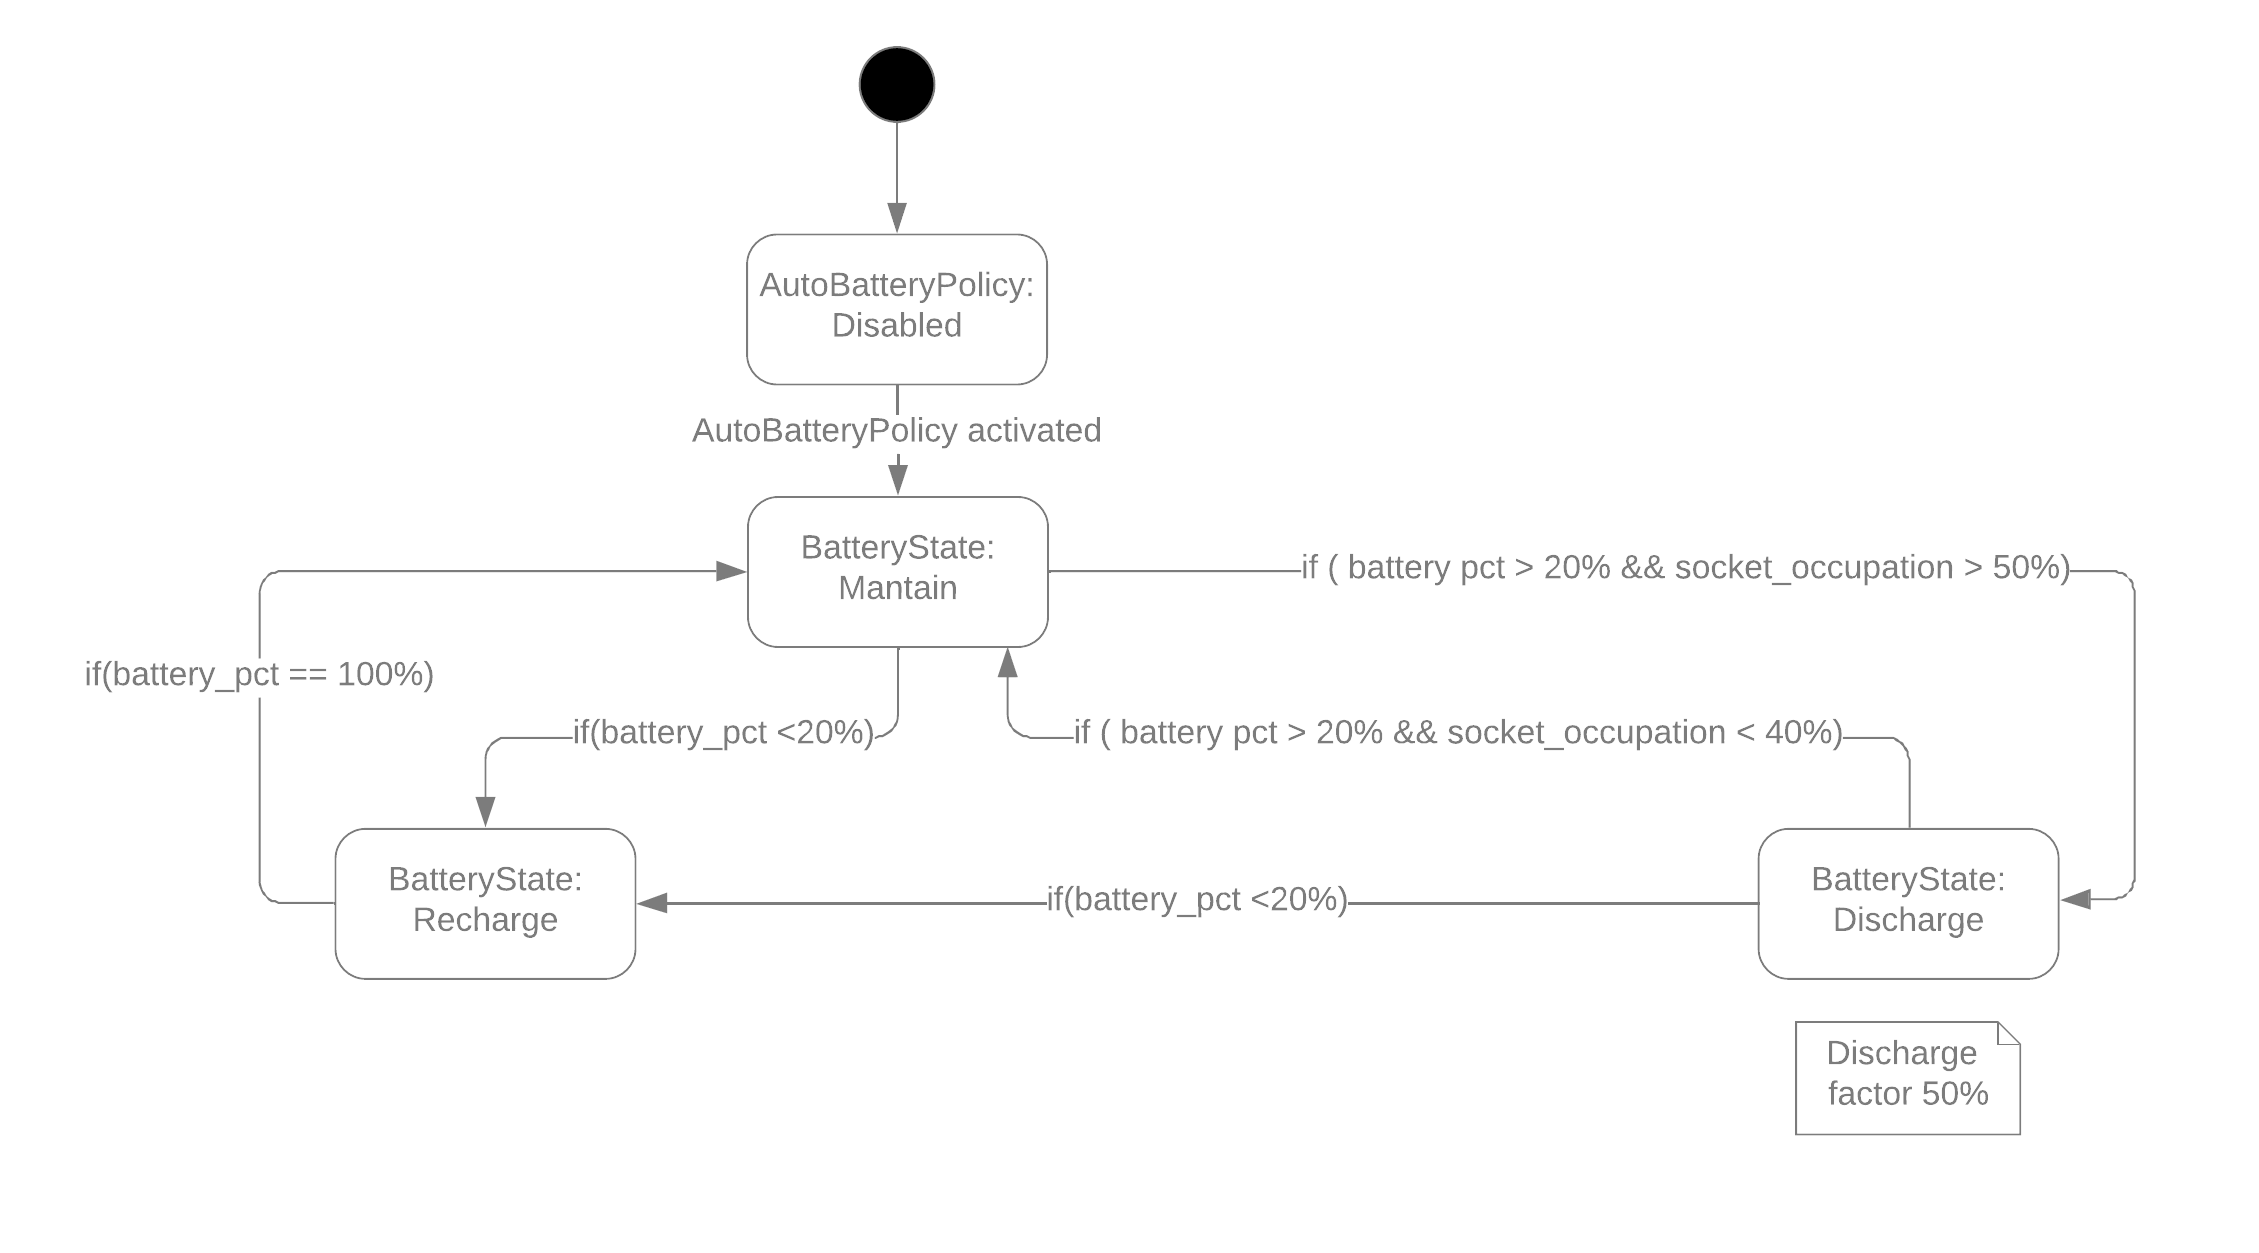
\includegraphics[width=\textwidth]{./img/battery_policy.png}
        \caption{Automatic battery policy state machine}
        \label{battery_policy}
    \end{figure}
\end{center}